\documentclass[12pt, a4paper]{article}
\usepackage[utf8]{inputenc} 
\usepackage[margin=1.2in]{geometry}
\usepackage{multicol}
\usepackage{multirow}
\usepackage{url}
\usepackage{graphicx}
\usepackage{amsfonts}
\usepackage[tbtags]{amsmath}
\usepackage{amsfonts,amssymb,amsmath,graphicx,hyperref}
\usepackage{tikz}
\usetikzlibrary{arrows}
\usepackage{caption}
\usepackage{subcaption}
\usepackage{float}
\usepackage{booktabs}
\usepackage{caption}
\usepackage{tikz}
\geometry{margin=1in}
\usepackage{enumitem}



\title{
	\line(1,0){300}
	\endgraf\bigskip
	\Huge
	\begin{center}
		\emph{\Large{\textbf{Tree of Thoughts Prompting}}}
		
	\end{center}
	\line(1,0){300}
	\bigskip
	\bigskip
}

\author{
        \textbf{Siam Ahamed}\\Student ID: 2105155\\
        \textbf{ Al Shahriar Alif}\\Student ID: 2105158\\
        \textbf{Imdadul Hasan}\\Student ID: 2105160\\\\
	Department of Computer Science and Engineering\\
    Bangladesh University of Engineering and Technology\\
}

\date{
	\endgraf\bigskip
	% {\today}
}
\begin{document}
	\maketitle
	\pagenumbering{roman}
    \pagebreak
    
    \tableofcontents
    \setcounter{tocdepth}{2}
    \newpage
        
    \listoffigures
    \newpage
        
    \listoftables
    \newpage
    
    
    \pagenumbering{arabic}
	%k=================================Siam====================================================

       \begin{abstract}
        In the rapidly evolving field of artificial intelligence and natural language processing, prompting techniques play a pivotal role in eliciting accurate and coherent responses from language models. This report explores the novel Tree of Thoughts (ToT) prompting technique, which structures reasoning into a tree-like framework, enabling systematic exploration of solution paths. Using the Game of 24\textemdash a challenging arithmetic problem requiring reasoning and creativity\textemdash we demonstrate the advantages of ToT prompting over traditional methods such as Input-Output (IO) Prompting, Chain-of-Thought (CoT) prompting, and Self-Consistency with CoT prompting. Through a comparative analysis, we highlight how ToT effectively leverages hierarchical problem-solving, leading to higher accuracy and better interpretability. This study underscores the potential of ToT prompting in enhancing complex reasoning tasks, paving the way for its broader application across domains requiring structured thought processes.
    \end{abstract}
	\section{Introduction}

Prompting techniques play a pivotal role in unlocking the reasoning capabilities of large language models (LLMs), enabling them to tackle complex tasks that require logic, creativity, and structured problem-solving. While traditional methods such as IO Prompting, Chain-of-Thought (CoT) prompting~\cite{COT}, and Self-Consistency with CoT~\cite{SE_TOC} have achieved significant success, they often fall short when addressing problems that require exploring multiple reasoning paths or navigating non-linear solution spaces. 

To address these challenges, the Tree of Thoughts (ToT) prompting framework~\cite{TOT} was introduced. By structuring the problem-solving process as a tree, ToT enables systematic exploration of alternative paths, fostering creativity and improving the model’s ability to reach accurate solutions.

This report evaluates the effectiveness of ToT prompting through the lens of the Game of 24, a mathematical puzzle that involves using four given numbers and basic arithmetic operations (addition, subtraction, multiplication, and division) to achieve a target value of 24. The problem demands both creativity and logical reasoning, making it an ideal benchmark for comparing prompting techniques. Specifically, we assess the performance of ToT prompting against IO Prompting, CoT prompting, and Self-Consistency with CoT prompting, providing insights into their strengths and limitations.

The remainder of this report is structured as follows: we introduce the Game of 24 as a representative problem, describe the prompting techniques under comparison, and later propose the ToT prompting framework. Finally, we present a detailed analysis of their performance.

\section{The Game of 24}

The Game of 24 is a mathematical reasoning challenge that tests logical thinking and creativity. The objective of the game is to combine four given numbers using basic arithmetic operations (\(+, -, \times, \div\)) to reach the target value of 24. The game encourages players to explore multiple ways of problem-solving, often requiring innovative and multi-step reasoning.

\subsection{Description of the Game}

The Game of 24 is simple in premise but challenging in execution:

\begin{itemize}
    \item \textbf{Goal:} Use four numbers and the four basic arithmetic operations to form an equation that equals 24.
    \item \textbf{Allowed Operations:} Addition (\(+\)), subtraction (\(-\)), multiplication (\(\times\)), and division (\(\div\)).
\end{itemize}

\textbf{Example:}
\begin{itemize}
    \item \textbf{Input Numbers:} 4, 9, 10, 13
    \item \textbf{Solution:} \((10 - 4) \times (13 - 9) = 24\)
\end{itemize}

This puzzle helps sharpen analytical thinking and demonstrates the importance of step-by-step reasoning when solving complex problems.

\section{Prompting Techniques to Solve the Game}

In this report, we explore different prompting techniques that can guide both humans and AI models in solving the Game of 24 effectively.

\subsection{Input-Output (IO) Prompting}

This technique establishes a direct relationship between the input (the numbers and operations) and the output (the solution). It works well for straightforward(just like the fig\ref{fig:IO-prompting} )  problems where minimal reasoning is needed.

\begin{figure}[h]
    \centering
    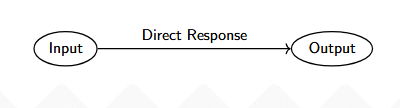
\includegraphics[width=0.7\textwidth]{IO.png}
    \caption{Input-Output Prompting.}
    \label{fig:IO-prompting}
\end{figure}

\textbf{Example:}
\begin{itemize}
    \item \textbf{Input:} 4, 4, 6, 8
    \item \textbf{Output:} \((8 - 6) \times (4 + 4) = 24\)
\end{itemize}

\textbf{Merits:}
\begin{itemize}
    \item Simple and easy to use.
    \item Faster response time.
    \item Ideal for basic arithmetic problems.
\end{itemize}

\textbf{Limitations:}
\begin{itemize}
    \item Limited to single-step reasoning.
    \item Fails in complex multi-step scenarios.
    \item Lacks contextual awareness.
\end{itemize}


\subsection{Chain of Thought (CoT) Prompting}
Unlike IO prompting, CoT prompting involves breaking down the problem into intermediate steps(In Fig \ref{fig:COT-prompting} ). It encourages multi-step reasoning and mimics how a human would think through the solution.
\begin{figure}[h]
    \centering    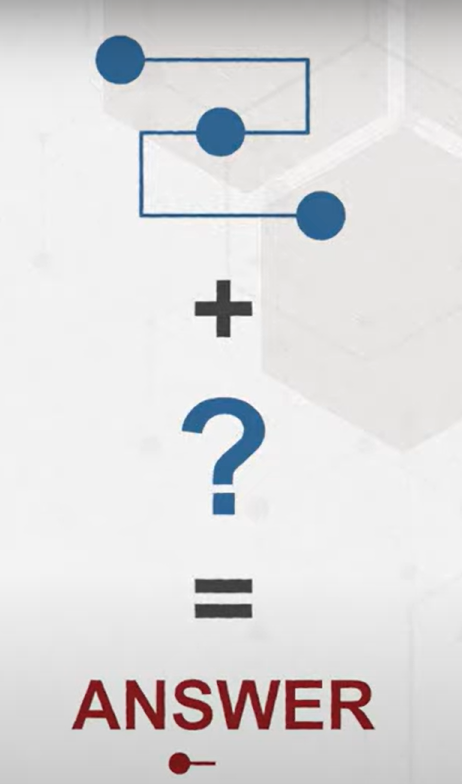
\includegraphics[width=0.7\textwidth,height=0.7\textwidth]{COT.png}
    \caption{Chain of Thought Prompting.}
    \label{fig:COT-prompting}
\end{figure}

\textbf{Process:}
\begin{enumerate}
    \item Identify sub-problems.
    \item Solve each step incrementally.
    \item Combine results to reach the final answer.
\end{enumerate}

\textbf{Example Solution with CoT:}
\begin{itemize}
    \item \textbf{Input:} 4, 4, 6, 8
    \item \textbf{Step 1:} Subtract 6 from 8: \(8 - 6 = 2\).
    \item \textbf{Step 2:} Add 4 and 4: \(4 + 4 = 8\).
    \item \textbf{Step 3:} Multiply results from steps 1 and 2: \(2 \times 8 = 24\).
\end{itemize}

\textbf{Merits:}
\begin{itemize}
    \item Handles complex problems effectively.
    \item Encourages logical reasoning.
    \item Achieves better accuracy in multi-step scenarios.
\end{itemize}
\subsection{Self-Consistency with Chain of Thought (CoT) Prompting}
Instead of generating a single chain of thought, the model generates multiple reasoning paths (solutions) for the same problem(Figure \ref{fig:SCOT-prompting}).
It then selects the final answer based on the most frequently reached conclusion across these diverse paths.
\begin{figure}[h]
    \centering
    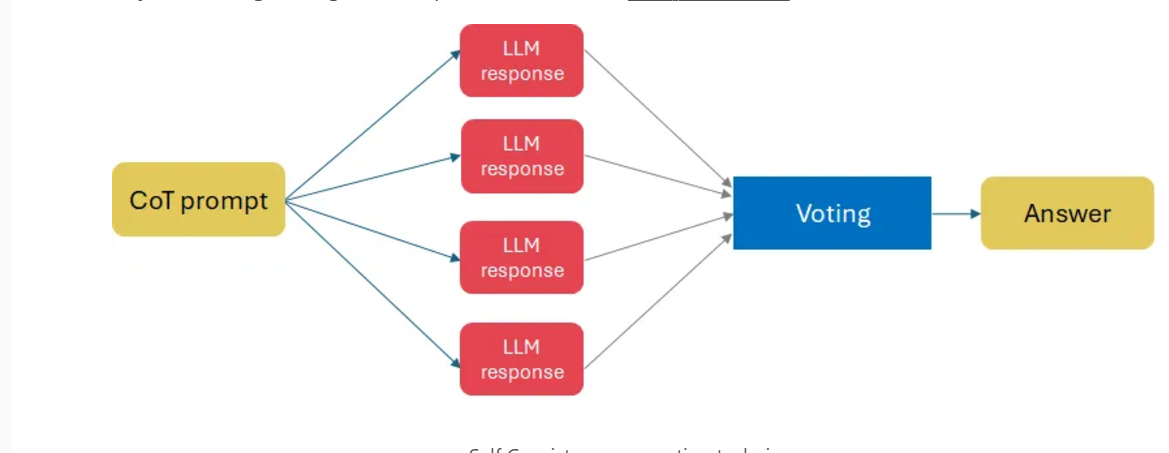
\includegraphics[width=\textwidth,height=0.7\textwidth]{STOC.png}
    \caption{Self-Consistency with Chain of Thought Prompting.}
    \label{fig:SCOT-prompting}
\end{figure}

\textbf{Process:}

\begin{enumerate}
    \item \textbf{Initiate with CoT/Few-shot Prompting}  
    \begin{itemize}
        \item Use examples to demonstrate reasoning patterns.  
        \item Begin with a well-structured prompt that encourages step-by-step reasoning.  
    \end{itemize}

    \item \textbf{Generate Multiple Outputs}  
    \begin{itemize}
        \item Instead of providing a single response, run the prompt multiple times.  
        \item Obtain a variety of plausible answers.  
    \end{itemize}

    \item \textbf{Select the Most Consistent Answer}  
    \begin{itemize}
        \item Aggregate all outputs from Step 2.  
        \item Choose the most frequent or consistent response as the final answer.  
    \end{itemize}
\end{enumerate}

\textbf{Example Solution with SC-CoT Prompting:} \\\\ 
\hspace{40pts}\textbf{  Input:} \{4, 4, 6, 8\}  

\begin{itemize}
    \item \textbf{Step 1:} Subtract \(6 - 4 = 2\)  
    \textbf{Remaining Numbers:} \{4, 8, 2\}  

    \item \textbf{Step 2:} Add \(4 + 8 = 12\)  
    \textbf{Remaining Numbers:} \{12, 2\}  

    \item \textbf{Step 3:} Multiply \(12 \times 2 = 24\)  
    \textbf{Final Result:} 24  
\end{itemize}

\textbf{Merits:}  
\begin{itemize}
    \item \textbf{Improved Accuracy and Reasoning:} Provides reliable solutions for complex problems.  
    \item \textbf{Supports Complex Problem Solving:} Encourages breaking challenges into manageable steps.  
    \item \textbf{Enhanced Explanations:} Solutions are clearer and more understandable.  
\end{itemize}

\textbf{Limitations:}  
\begin{itemize}
    \item \textbf{Scalability Challenges:} Requires multiple iterations, increasing computational cost.  
    \item \textbf{Vulnerability to Intermediate Errors:} Incorrect steps may lead to erroneous outputs.  
    \item \textbf{Resource Intensive:} Demands additional processing time and resources.  
\end{itemize}


\textbf{Limitations:}
\begin{itemize}
    \item Slower than IO prompting.
    \item Requires structured instructions.
\end{itemize}


\section{Comparison of Techniques}

\begin{table}[H]
    \centering
    \begin{tabular}{@{}p{3.5cm}p{6.5cm}p{6.5cm}@{}}
    \toprule
    \textbf{Technique}       & \textbf{Merits}                                & \textbf{Limitations}                         \\
    \midrule
    IO Prompting             & Quick and simple for single-step problems.     & Struggles with complex or multi-step reasoning tasks. \\
    Chain of Thought (CoT)   & Enables step-by-step reasoning, improving logical accuracy. & Slower due to sequential steps and lacks robustness in branching decision-making. \\
    Self-Consistency with CoT & Enhances accuracy by aggregating multiple reasoning paths. & Computationally expensive and limited in handling diverse solution spaces. \\
    \bottomrule
    \end{tabular}
    \caption{Comparison of Prompting Techniques.}
    \label{tab:techniques-comparison}
\end{table}

So we see existing techniques fall short when faced with problems that require systematic exploration of diverse pathways and iterative decision-making, as seen in human problem-solving. Tree of Thought (ToT) prompting addresses these limitations by:
\begin{itemize}
    \item Encouraging exploration of multiple branches of reasoning simultaneously.
    \item Adopting a hierarchical structure to evaluate and prune solutions, similar to how humans reason through complex scenarios.
    \item Providing a more comprehensive and adaptable approach to solving problems like the Game of 24, where intermediate decisions significantly impact the final outcome.
\end{itemize}

ToT prompting not only mirrors human thinking but also introduces a scalable framework for tackling problems involving intricate reasoning and decision trees, making it the ideal technique for our next exploration.


\section{Understanding Human Problem-Solving and Structured Thinking}
Human problem-solving methods can be broadly classified into two categories:
\begin{enumerate}
    \item \textbf{Random Thinking:} A spontaneous and unstructured approach often adopted by common individuals.
    \item \textbf{Structured Thinking:} A logical and well-organized approach characteristic of mathematicians and systematic thinkers.
\end{enumerate}
    This part of the report analyzes these approaches, demonstrating their strengths and weaknesses through examples and applying them to AI modeling.
\subsection{Methods}
\subsubsection{Random Thinking and Its Limitations}
\textbf{Definition:}Random thinking involves trial-and-error methods without a coherent strategy.\\
\textbf{Example:}  Solving the "Game of 24" with numbers :
\begin{enumerate}
    \item Choose 14 and 3  and multiply them to get  42.
    \item Divide 42  by 7, resulting in 6 .
    \item Multiply 6 with 3 to get 18, which is not the target 24.
    
\end{enumerate}
\textbf{Limitation:} Random approaches often lead to failure as they lack a systematic pathway to the solution.
\subsubsection{Structured Thinking by Mathematicians}
\textbf{Definition:} Structured thinking involves logical steps to decompose and solve a problem.\\
\textbf{Example:} Solving the "Game of 24" systematically:
\begin{enumerate}
    \item \textbf{Sorting Inputs:} Arrange numbers .
    \item \textbf{Initial Evaluation:}
    \begin{itemize}
        \item Check if any number exceeds : None.
        \item Multiply all numbers to confirm a solution is possible: .
    \end{itemize}
    \item \textbf{Logical Exploration:}
    \begin{itemize}
        \item Identify promising operations (e.g., $5*7=35$,$14-3=11$ ).
        \item Subtract 11 from 35  to reach 24.
    \end{itemize}
\end{enumerate}
\begin{figure}[H]
    \centering
    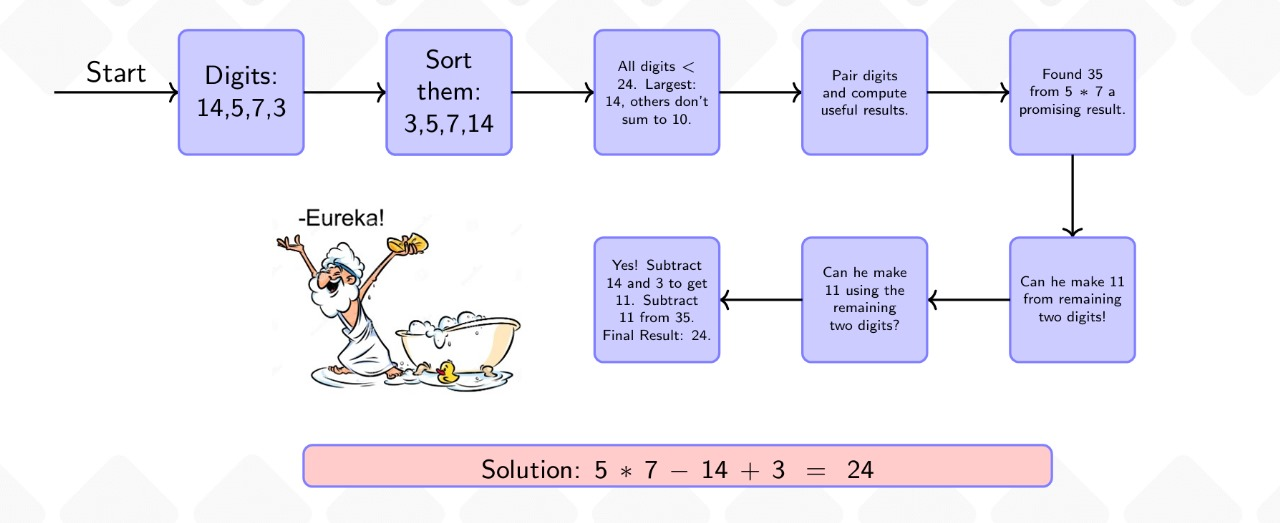
\includegraphics[width=\textwidth,height=0.5\textwidth]{WhatsApp Image 2024-12-30 at 22.12.38_3ff0e297.jpg}
    \caption{Solving Game of 24 using structured thinking}
    \label{fig:Solving game iof 24.}
\end{figure}
\textbf{Result:} Solution achieved efficiently through logical steps.

\subsection{Results}
\subsubsection{Key Observations}
\begin{enumerate}
    \item \textbf{Random Thinking:}
    \begin{itemize}
        \item Inefficient and prone to errors.
        \item May succeed occasionally but lacks reliability.
    \end{itemize}
    \item \textbf{Structured Thinking:}\begin{itemize}
        \item Eliminates unnecessary calculations.
        \item Guarantees a solution when possible through logical exploration.
    \end{itemize}
\end{enumerate}
\subsection*{Visualization of Process}
\begin{table}[H]
\centering
\begin{tabular}{|l|l|l|}
\hline
Step & Action                 & Result            \\ \hline
1    & Sort inputs            &                   \\ \hline
2    & Evaluate Possibilities & Solution Possible \\ \hline
3    & Logical Operations     &                   \\ \hline
4    & Final Calculation      &                   \\ \hline
\end{tabular}
\caption{Structured Thinking.}
    \label{tab:Thinking procedure}
\end{table}
\section{Application to AI: Modeling Human Problem-Solving}
\subsection{Tree of Thought (ToT) Prompting}
ToT is an AI methodology inspired by structured human thinking. It includes the following steps:
\begin{enumerate}
    \item \textbf{Problem Decomposition:} Break down the problem into smaller components.
    \item \textbf{Thought Generation:} Explore possible solutions using logical operations.

    \item \textbf{State Evaluation:} Assess intermediate results for progress toward the goal.
    \item \textbf{Decision Making:} Select the most promising path to reach the solution.


\end{enumerate}


\subsection{Example: AI Solving "Game of 24"}
\begin{enumerate}
    \item \textbf{Problem Decomposition:}
    \begin{itemize}
        \item Numbers:3,5,7,14.
        \item Target: 24.
        \item Pair the inputs.
        \begin{figure}[H]
    \centering
    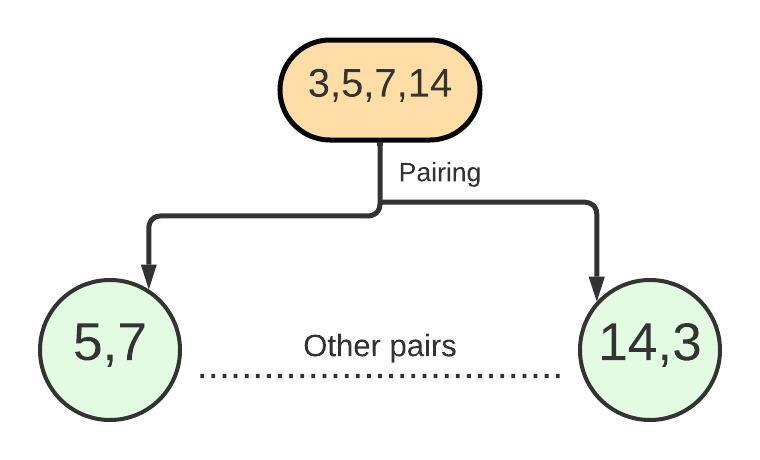
\includegraphics[width=0.45\textwidth,height=0.35\textwidth]{Org chart.jpeg}
    \caption{Pairing Inputs}
    \label{fig:Pairing Inputs.}
\end{figure}
    \end{itemize}
    \item \textbf{Thought Generation:}
    \begin{itemize}
        \item Systematically compute results from the pairs generated in the decomposition
  step and apply operations to approach the target 24.
  \item From the decomposition step , pairs such as (5,7) and (14,3) are identified.
  \item Different arithmetic operations are performed on these pairs to generate intermediate values.
  \item For example:
   \begin{figure}[H]
    \centering
    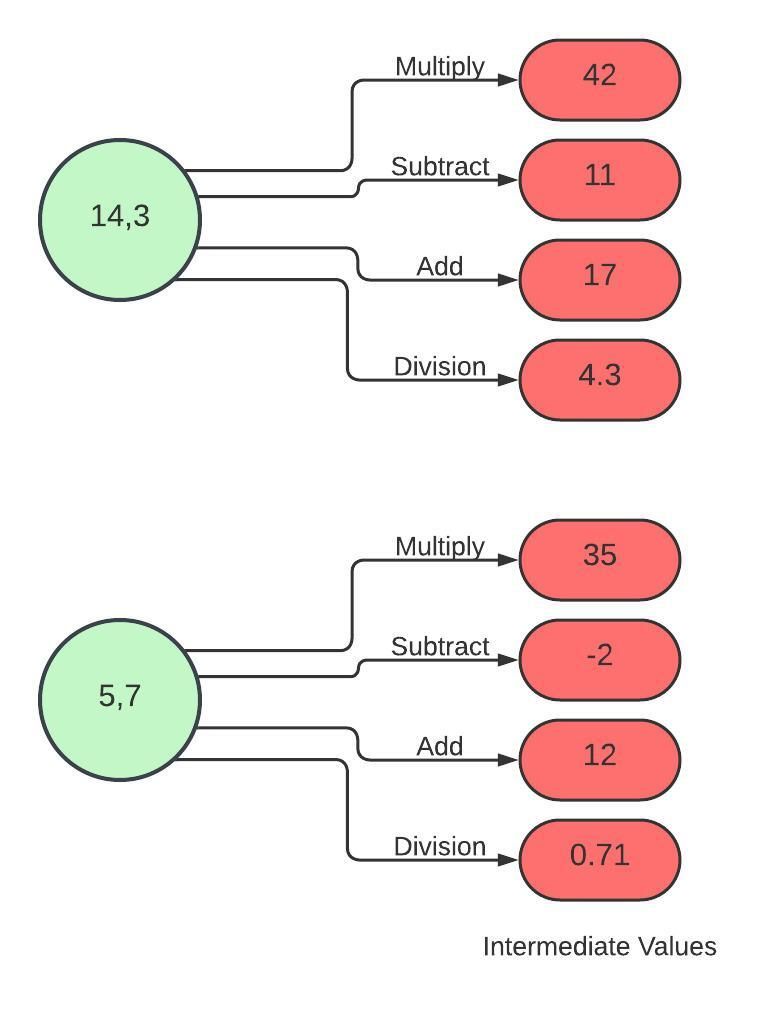
\includegraphics[width=0.5\textwidth,height=0.5\textwidth]{Org chart (1).jpeg}
    \caption{Performing Arithmetic Operations on Paired Values to Generate Intermediate Values.}
    \label{fig:Generating Intermediate Values}
\end{figure}
    \end{itemize}
    \item \textbf{State Evaluation:}\begin{itemize}
        \item Evaluate  as promising.
        \item Check if  can be formed from remaining numbers.
    \end{itemize}
    \item \textbf{Decision Making:}
    \begin{itemize}
        \item Combine results to achieve .
    \end{itemize}
    
\end{enumerate}
\section{Advantages of Structured Thinking}
\begin{enumerate}
    \item \textbf{Efficiency: }Reduces unnecessary calculations and random guesses.
    \item \textbf{Reliability: }Ensures a logical path to the solution.
    \item \textbf{Applicability: }Can be extended beyond puzzles to real-world problems.
\end{enumerate}


\section{Solving Game of 24 Using Tree of Thought (ToT)}

\bigskip

\subsection{Conceptual Stages or Processes of Tree of Thought (ToT) Prompting}

Tree of Thought (ToT) prompting involves breaking down problem-solving into two key processes: \textbf{Propose Prompt} and \textbf{Value Prompt}. These stages enable systematic exploration of potential solutions and evaluation of their validity, guiding a language model (LM) through reasoning like a human would while solving complex problems.

\bigskip
% \line(1,0){\textwidth}
\bigskip

\begin{figure}[H]
    \centering
    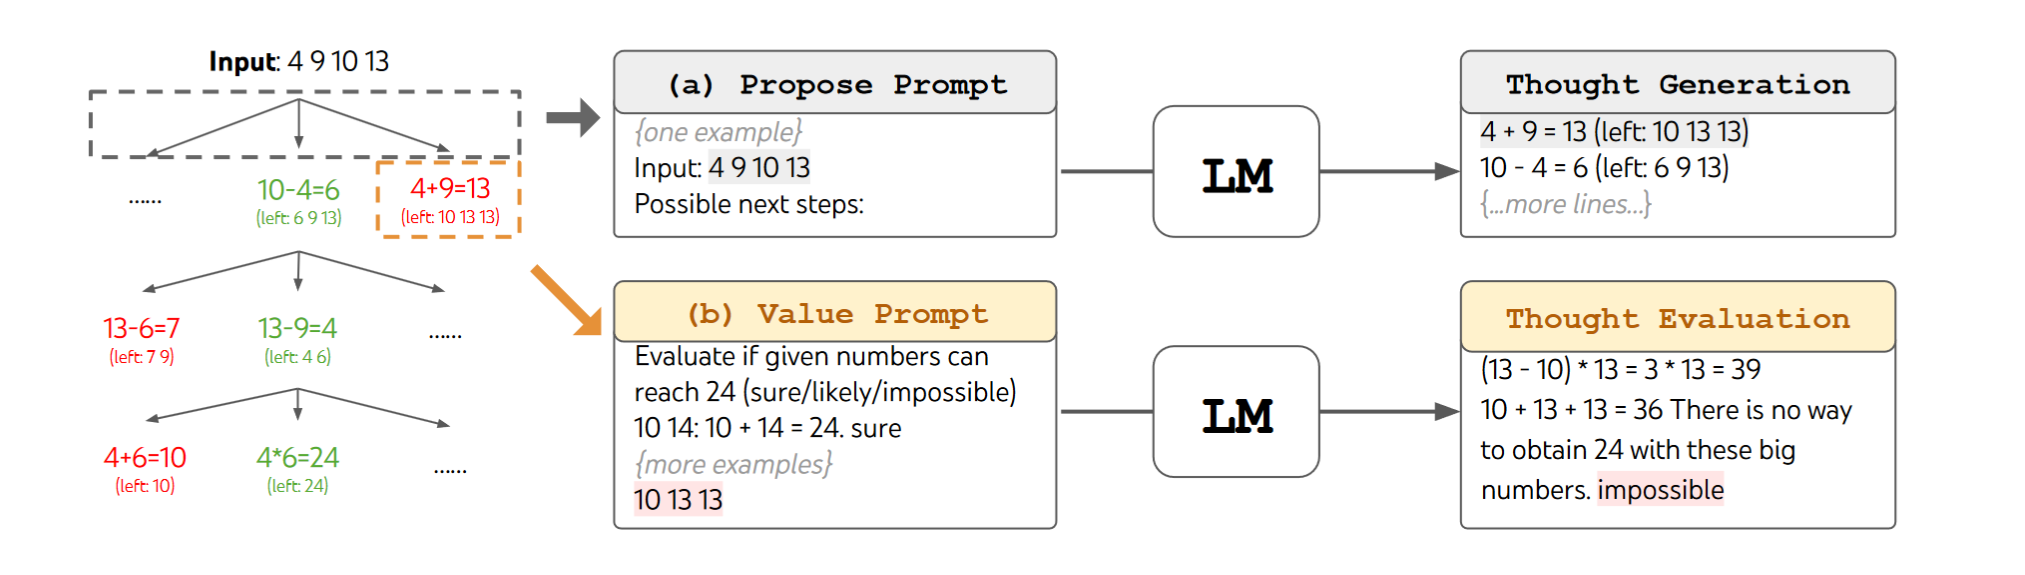
\includegraphics[width=\textwidth,height=0.45\textwidth]{game24sol.png}
    \caption{ ToT in a game of 24. The LM is prompted for (a) thought generation and (b) valuation}
    \label{fig:g24.}
\end{figure}



\begin{enumerate}

    \item \textbf{Propose Prompt (Thought Generation)} \\
    \textbf{Objective:} To generate possible next steps or ideas that lead closer to the solution of a problem.
    
    \textbf{Key Characteristics:}
    \begin{itemize}
        \item \textbf{Exploration:} The LM is prompted to think of multiple possible actions or operations based on the current input or state.
        \item \textbf{Tree Structure:} Each proposed step creates a ``branch'' in a tree, representing a new state in the reasoning process.
        \item \textbf{Open-ended Generation:} Encourages exploration of all viable options, expanding the solution space.
    \end{itemize}
    
    \textbf{Example:}
    In the \textit{Game of 24}, given the input numbers 4, 9, 10, 13, the Propose Prompt might ask: \\
    \textit{``What operations can be performed on these numbers to move closer to the target value of 24?''}
    
    The LM might generate:
    \begin{itemize}
        \item $4 + 9 = 13$ (new state: \{13, 10, 13\})
        \item $10 - 4 = 6$ (new state: \{6, 9, 13\})
    \end{itemize}
    
    This step focuses on what could be done next, creating a roadmap of possibilities.

    \item \textbf{Value Prompt (Thought Evaluation)} \\
    \textbf{Objective:} To evaluate the feasibility or desirability of a particular branch or idea in the solution tree.
    
    \textbf{Key Characteristics:}
    \begin{itemize}
        \item \textbf{Judgment:} The LM assesses whether the current state is likely, unlikely, or certain to lead to the solution.
        \item \textbf{Pruning the Tree:} Irrelevant or unproductive paths are discarded, allowing focus on promising branches.
        \item \textbf{Qualitative Assessment:} Results are categorized into labels such as:
        \begin{itemize}
            \item \textbf{Sure:} The solution can be achieved from this state.
            \item \textbf{Likely:} The solution may be possible, but further steps are needed.
            \item \textbf{Impossible:} The solution cannot be achieved from this state.
        \end{itemize}
    \end{itemize}
    
    \textbf{Example:}
    For the \textit{Game of 24}, given the state \{10, 13, 13\}, the Value Prompt might ask: \\
    \textit{``Can these numbers be combined to reach 24?''}
    
    The LM evaluates:
    \begin{itemize}
        \item $10 + 13 + 13 = 39 \rightarrow$ \textbf{Impossible}, as there is no way to reduce this to 24.
    \end{itemize}
    
    This step focuses on whether the current idea works or is worth pursuing further.

\end{enumerate}
\bigskip
The fig \ref{fig:example} demonstrates a "Tree of Thought" prompting technique to solve the arithmetic expression (5 * 7) - 14 + 3 using the input numbers 3, 5, 7, 14. It shows a computation tree where each node represents an intermediate step, applying arithmetic operations such as addition, subtraction, multiplication, or division to pairs of numbers. Valid operations producing integer results are expanded further, while invalid paths, such as non-integer division results, are discarded. The tree systematically explores all possible computation paths, breaking down the problem into smaller subproblems. The successful path leading to the final result is highlighted with red arrows, showcasing the reasoning process behind solving the problem.
\begin{figure}[h!]
    \centering
    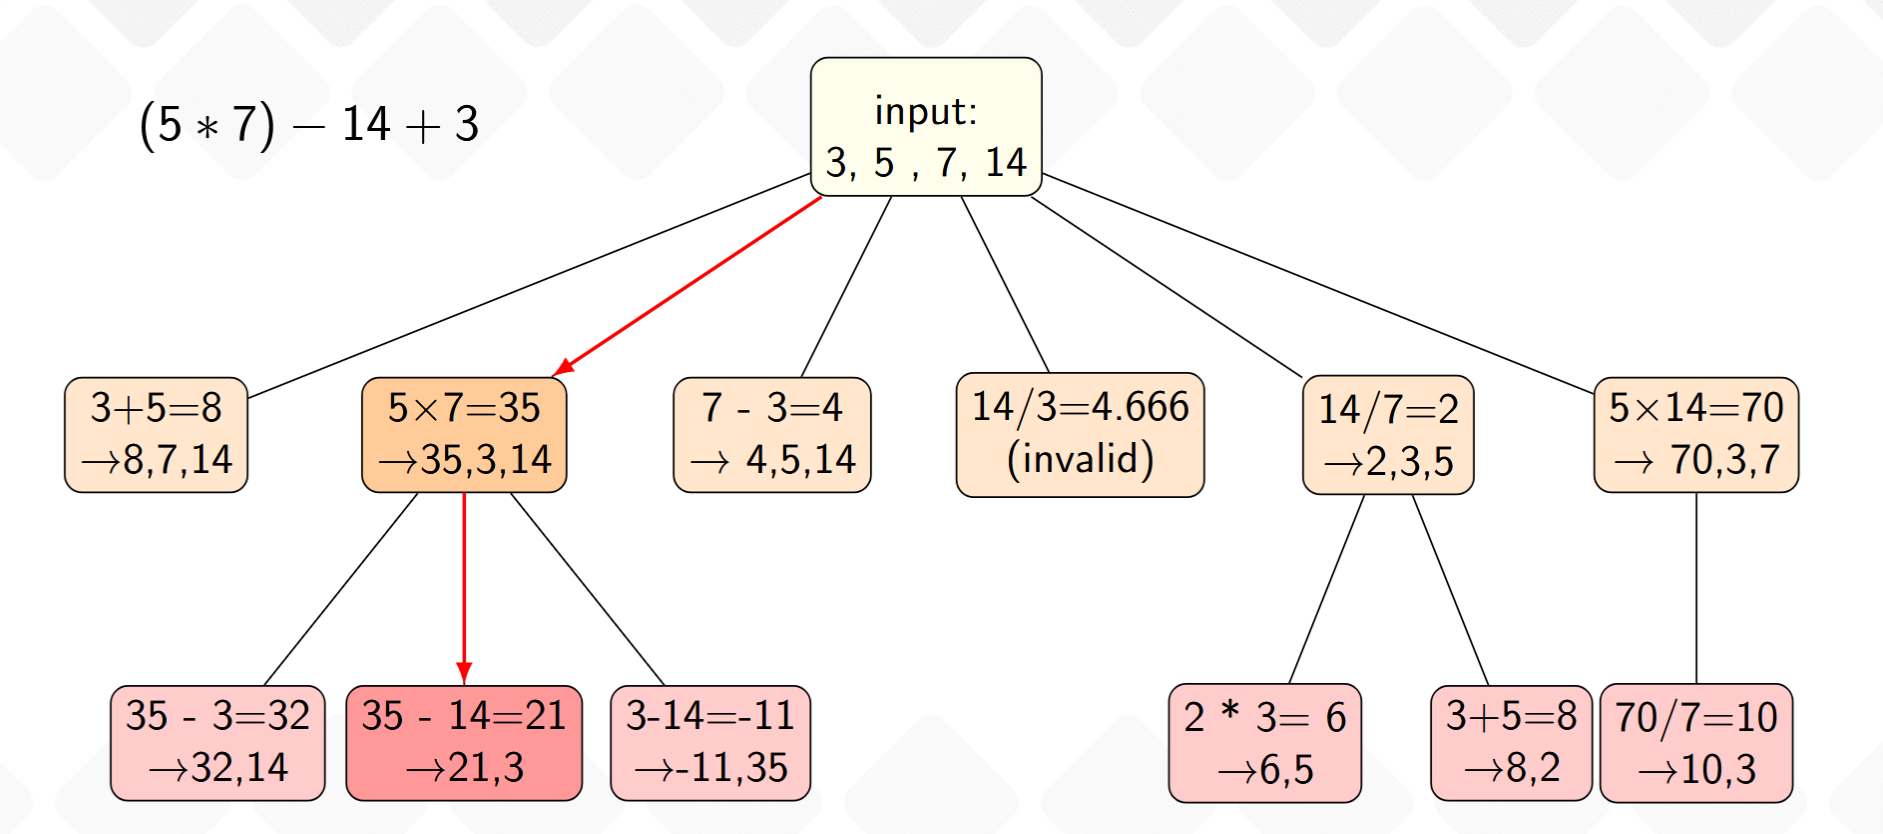
\includegraphics[width=0.95\textwidth]{game24_example.png} 
    \caption{Visualization of game of 24}
    \label{fig:example}
\end{figure}
\pagebreak

\section{Conclusion}
The experiments conducted on Tree of Thought (ToT) prompting in solving Game of 24 problems demonstrate its potential to systematically explore and evaluate multiple reasoning paths, mirroring human problem-solving processes. By leveraging intermediate steps and decision-making at each node, ToT enhances problem-solving accuracy, particularly in tasks involving logical reasoning, planning, and decision-making.

\subsection{Capabilities}
Tree of Thought prompting exhibits several strengths:
\begin{itemize}
\item \textbf{Enhanced Accuracy:} Compared to traditional methods like Chain of Thought (CoT) reasoning, ToT achieves a significantly higher success rate, as evidenced by its 74\% success in solving Game of 24 problems.
\item \textbf{Structured Exploration:} By systematically branching and evaluating multiple solution pathways, ToT enables deliberate exploration of complex problems, leading to more reliable outcomes.
\item \textbf{Broad Applicability:} While particularly effective in structured reasoning tasks, this approach holds promise across a variety of domains requiring systematic problem-solving.
\end{itemize}

\subsection{Limitations}
Despite its advantages, ToT prompting has notable limitations:
\begin{itemize}
\item \textbf{Resource Intensity:} As shown in the cost analysis (Table ~\ref{tab:cost_analysis}), ToT requires a high number of generated and prompt tokens, resulting in greater computational costs compared to other methods.
\begin{table}[h!]
\centering
\resizebox{.8\textwidth}{!}{%
\begin{tabular}{|l|c|c|c|}
\hline
\textbf{Method} & \textbf{Generate/Prompt Tokens} & \textbf{Cost per Case} & \textbf{Success Rate} \\ \hline
IO (best of 100) & 1.8k / 1.0k & \$0.13 & 33\% \\ \hline
CoT (best of 100) & 6.7k / 2.2k & \$0.47 & 49\% \\ \hline
ToT & 5.5k / 1.4k & \$0.74 & 74\% \\ \hline
\end{tabular}%
}
\caption{Cost analysis on Game of 24.}
\label{tab:cost_analysis}
\end{table}
\item \textbf{Task Specificity:} The approach is best suited for tasks requiring structured and logical problem-solving, limiting its applicability to less structured or highly creative tasks.
\end{itemize}


\bigskip


\subsection*{Relevance to AI Advancements}
The structured problem-solving paradigm exemplified by Tree of Thought prompting represents a significant step forward for AI systems. By improving reasoning capabilities and enabling efficient solution pathways, this approach contributes to advancing AI's ability to tackle complex, multi-step problems. While resource demands and limited task generality present challenges, ongoing optimization efforts could broaden its usability and cost-effectiveness.


    \pagebreak
    \footnotesize{
        \begin{thebibliography}{99}
        
            \bibitem{COT} 
            Jason Wei, Xuezhi Wang, Dale Schuurmans, Maarten Bosma, Brian Ichter, Fei Xia, Ed Chi, Quoc Le, Denny Zhou.
            \textit{ "Chain-of-Thought Prompting Elicits Reasoning in Large Language Models."}
            Submitted on 28 Jan 2022 
            
            \bibitem{SE_TOC} 
            Xuezhi Wang, Jason Wei, Dale Schuurmans, Quoc Le, Ed Chi, Sharan Narang, Aakanksha Chowdhery, Denny Zhou.
            \textit{ Self-Consistency Improves Chain of Thought Reasoning in Language Models.}
            Published at ICLR 2023. V2: added PaLM results; V3: added UL2 results; V4: camera ready version at ICLR 2023.
            
            \bibitem{TOT} 
            Shunyu Yao, Dian Yu, Jeffrey Zhao, Izhak Shafran, Thomas L. Griffiths, Yuan Cao, Karthik Narasimhan.
            \textit{Tree of Thoughts: Deliberate Problem Solving with Large Language Models.}
            NeurIPS 2023 camera ready version..
            
        \end{thebibliography}
    }
\end{document}

